\begin{mydef}
	Deux figures sont \kw{\hspace*{4cm} par rapport à une droite $(d)$} si elles se superposent quand on plie le long de cette droite. 
	La droite $(d)$ est appelée \kw{\hspace*{5cm}}.

\end{mydef}




\begin{myex}
	\begin{center}
		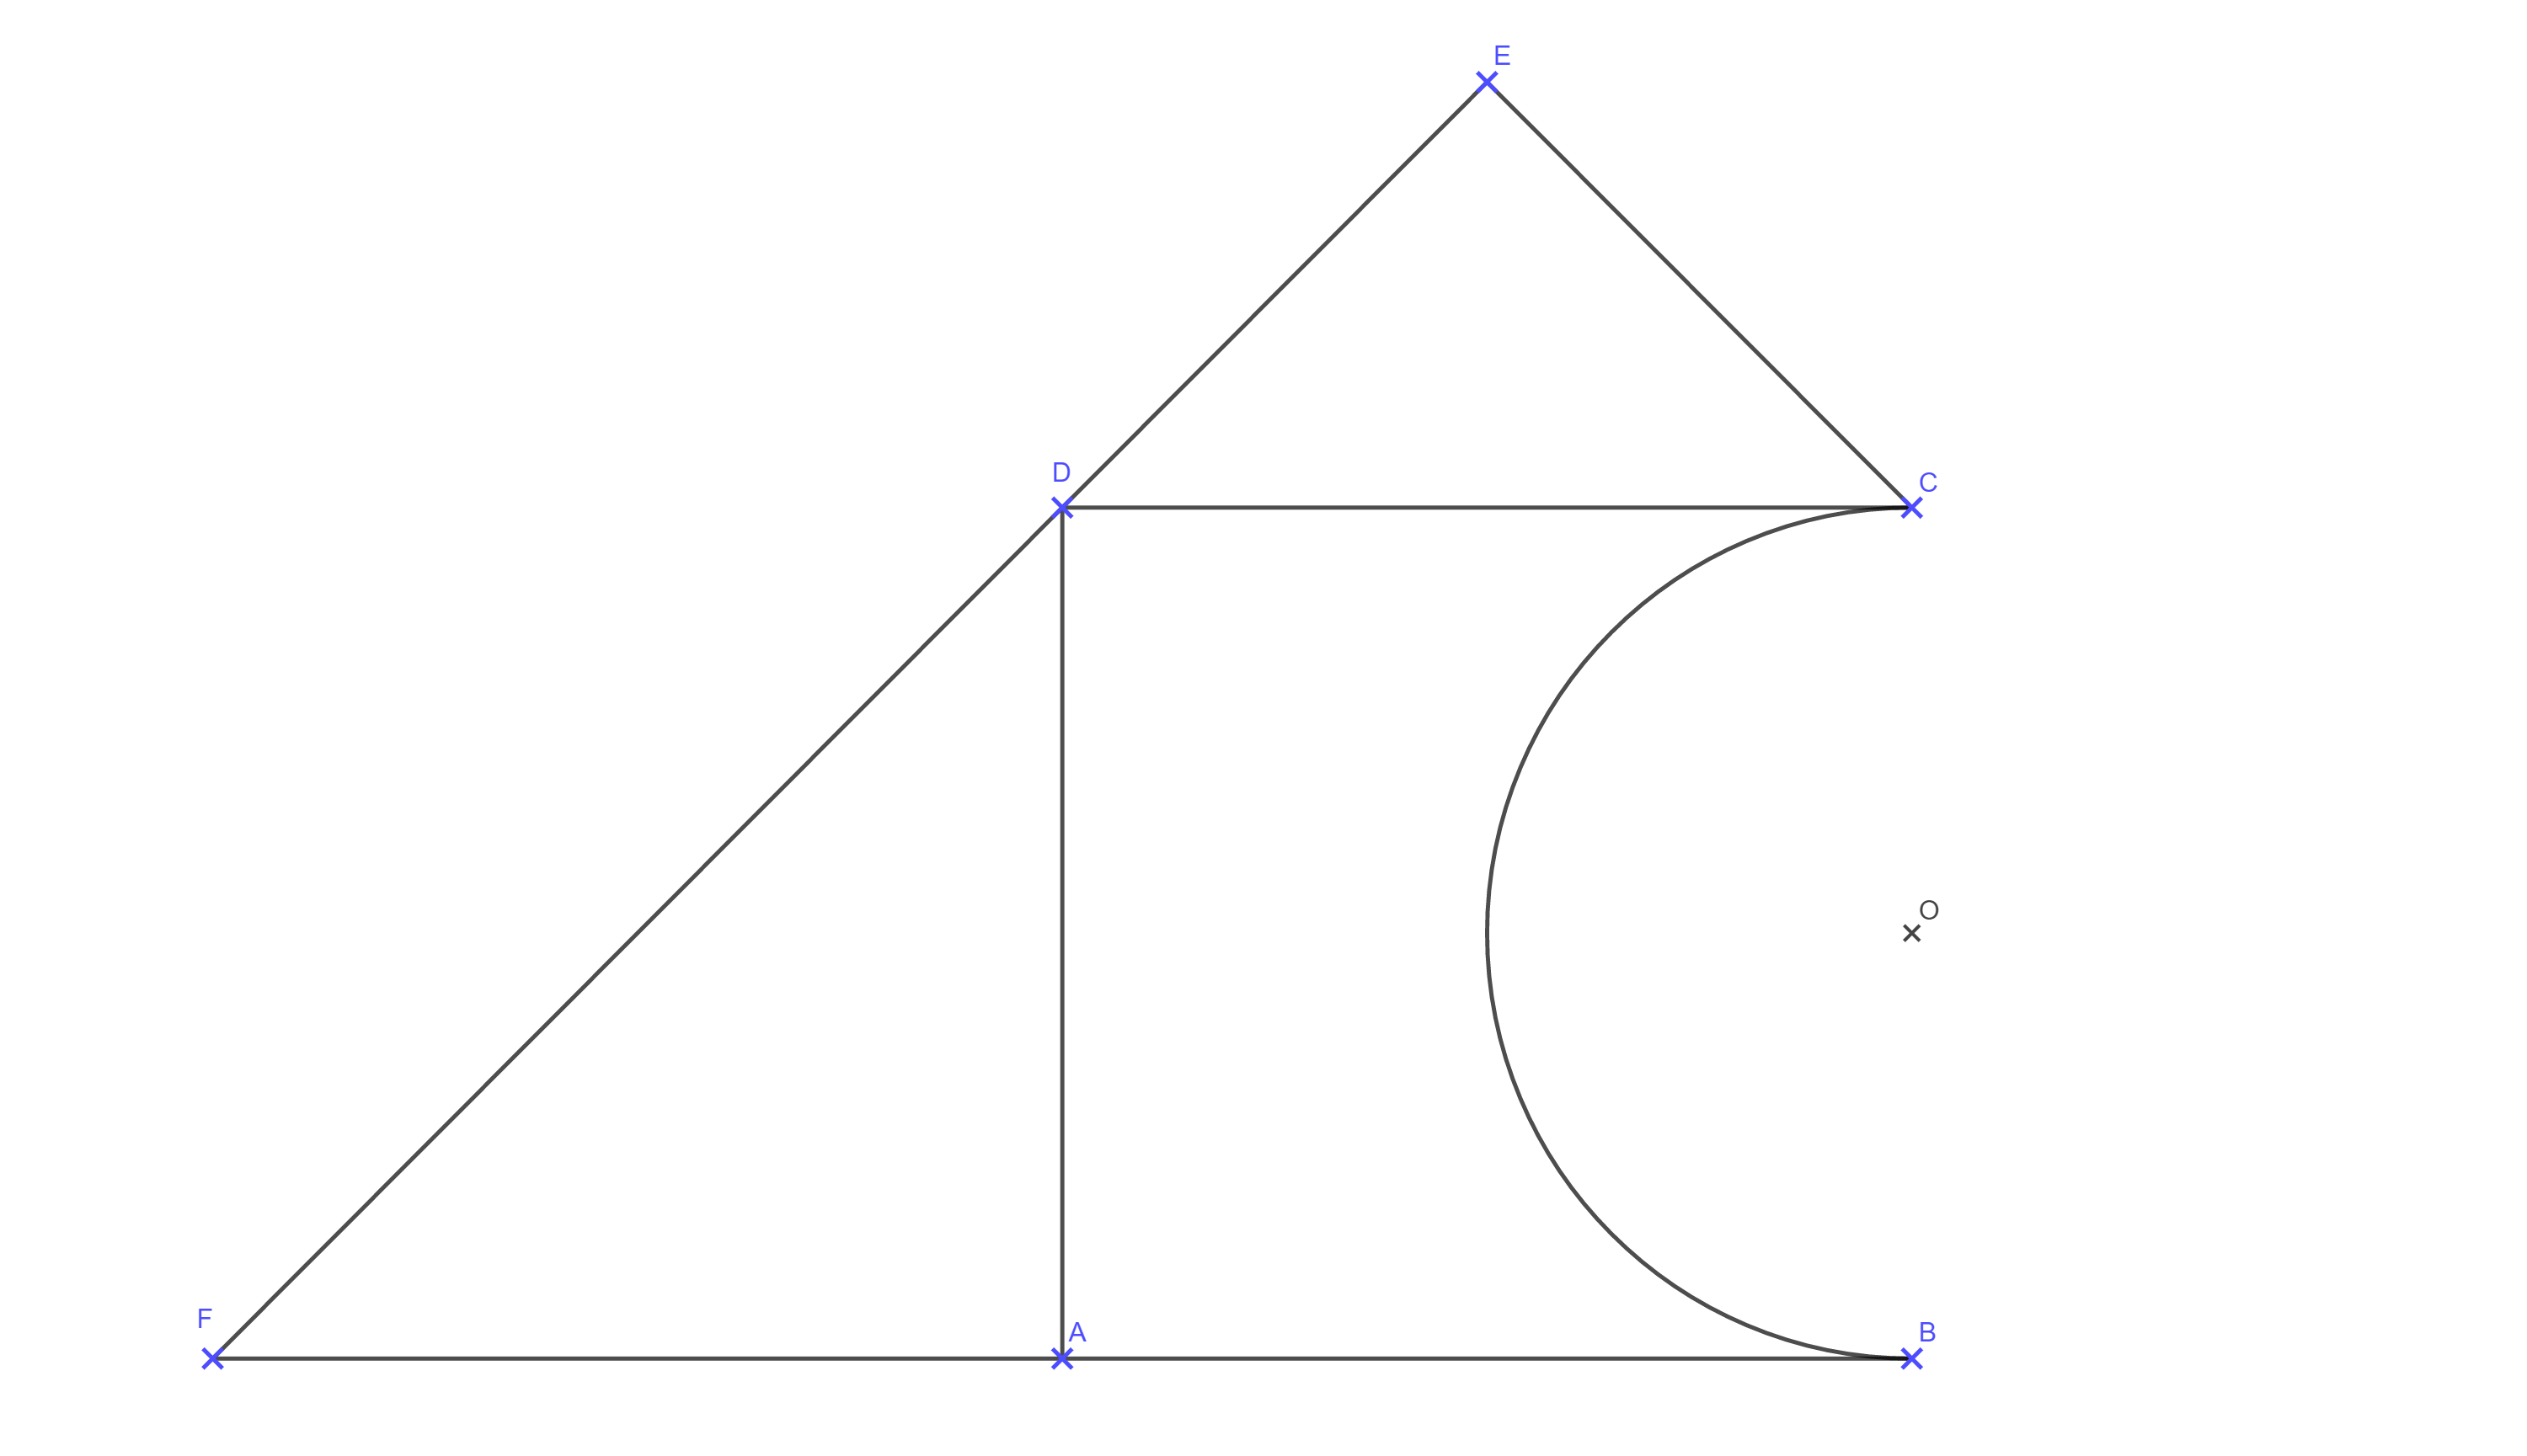
\includegraphics[scale=.8]{fig1}
	\end{center}	
\end{myex}

\begin{multicols}{2}
	
	\begin{center}
		\includegraphics*[scale=0.25]{def}
	\end{center}
	
	\begin{myprops}
		Soit $(d)$ une droite :
		\begin{itemize}
			\item Si un point $A$ n'appartient pas à la droite $(d)$, alors son symétrique par rapport à la droite $(d)$ est le point $A'$ tel que \kw{$(d)$ est la \hspace*{5cm}} \hspace*{5cm}.
			\item Si un point $B$ appartient à la droite $(d)$, alors son symétrique par rapport à la droite $(d)$ est \hspace*{4cm}.
		\end{itemize}
	\end{myprops}
	
	
\end{multicols}
